%% ============================================================================
%%  VERA: Vision-Experience-Reasoning-Action
%%  CoRL 2026 Camera-Ready Submission
%%  Authors: Sara Aly
%%
%%  Required files in the same directory as this .tex:
%%    corl_2026.sty       — from the CoRL 2026 template package
%%    corlabbrvnat.bst    — from the CoRL 2026 template package
%%    references.bib      — your bibliography database
%%    VERA.png            — architecture figure
%% ============================================================================
\documentclass{article}

%% CoRL 2026 camera-ready style.
%%   [final]    = camera-ready: named authors + conference footer (USE FOR SUBMISSION)
%%   [preprint] = preprint (e.g., arXiv): named authors, no footer
%%   (none)     = blind review: anonymous + "Submitted to …" footer + line numbers
\usepackage[final]{corl_2026}
%% NOTE: corl_2026.sty automatically loads natbib [square,numbers],
%%       hyperref, and geometry — do NOT load those packages again here.

%% ── Encoding & fonts ─────────────────────────────────────────────────────────
\usepackage[utf8]{inputenc}
\usepackage[T1]{fontenc}
%% (The style sets Times Roman as the main font via \rmdefault=ptm.)

%% ── Math ─────────────────────────────────────────────────────────────────────
\usepackage{amsmath,amssymb,amsfonts,mathtools,amsthm}

%% ── Figures ──────────────────────────────────────────────────────────────────
\usepackage{graphicx,wrapfig,float,subcaption,adjustbox}

%% ── Tables ───────────────────────────────────────────────────────────────────
\usepackage{booktabs,multirow,tabularx,array,colortbl,makecell}
\newcolumntype{L}[1]{>{\raggedright\arraybackslash}p{#1}}
\newcolumntype{C}[1]{>{\centering\arraybackslash}p{#1}}
\renewcommand{\arraystretch}{1.25}

%% ── Text & lists ─────────────────────────────────────────────────────────────
\usepackage{nicefrac,microtype,enumitem,scalefnt,xspace}

%% ── Colour ───────────────────────────────────────────────────────────────────
\usepackage{xcolor}
\definecolor{NewOrange}{HTML}{E67E22}
\definecolor{CodeBg}{HTML}{F8F9FA}
\definecolor{BorderGray}{HTML}{D1D5DB}

%% ── Listings ─────────────────────────────────────────────────────────────────
\usepackage{listings,pifont}
\lstdefinestyle{mycode}{
  basicstyle=\ttfamily\footnotesize,
  backgroundcolor=\color{CodeBg},
  frame=single, rulecolor=\color{BorderGray},
  breaklines=true, showstringspaces=false,
  aboveskip=4pt, belowskip=4pt,
}
\lstset{style=mycode}

%% ── Cross-references (must come after hyperref, which corl_2026 loads) ───────
\usepackage[capitalize,noabbrev]{cleveref}

%% ── PDF metadata ─────────────────────────────────────────────────────────────
%% The pdftitle MUST match the title on the OpenReview submission form.
\hypersetup{
  pdftitle  = {VERA: Closed-Loop Feedback for Grounded Vision-Action Policies
               via Experience and Reasoning},
  pdfauthor = {Sara Aly},
}

%% ── Macros ───────────────────────────────────────────────────────────────────
\newcommand{\cmark}{\ding{51}}
\newcommand{\xmark}{\ding{55}}
\newcommand{\modelname}{\textsc{VERA}\xspace}
\newcommand{\Lact}{$E_{\mathrm{act}}$\xspace}
\newcommand{\Lexp}{$E_{\mathrm{exp}}$\xspace}
\newcommand{\Lcon}{\Lexp}
\newcommand{\NEW}{\textcolor{NewOrange}{\textbf{[new]}}\xspace}
\newcommand{\tbd}{\textit{---}\xspace}
\newcommand{\veraresult}[2]{$#1\,{\pm}\,#2$}

%% ============================================================================
%%  Title — must match OpenReview exactly (same string as pdftitle above)
%% ============================================================================
\title{VERA: Closed-Loop Feedback for Grounded Vision-Action Policies
       via Experience and Reasoning}

%% Authors — non-anonymous; visible because [final] is active.
\author{
  Sara Aly\\
  Department of Computer Science\\
  California State University, Northridge\\
  United States\\
  \texttt{sarakhaledsea@gmail.com}
}

\begin{document}
\maketitle

%% ============================================================================
\begin{abstract}
Standard Vision-Language-Action (VLA) models treat each decision as a
stateless function of the current camera frame and task instruction,
discarding two informative signals that arise from prior interaction:
\emph{(i)} what action the agent attempted at the previous step, and
\emph{(ii)} whether that action moved it closer to the goal.
We present \modelname\ (Vision-Experience-Reasoning-Action), a
five-stream closed-loop robot policy that continuously re-injects both
signals back into the decision process.
The previous action is narrated from a fixed vocabulary and
re-encoded as an action narration token \Lact\ through the frozen CLIP
encoder, gated by the received reward so successful actions speak
louder than failed ones.
The observed outcome---reward and signed distance-to-goal delta---is
jointly verbalized into one of up to 16 semantically distinct strings
and re-encoded as an experience token \Lexp\ \NEW, capturing
\emph{what happened} orthogonally to \emph{what was attempted}.
A rolling window of low-level continuous action vectors, discrete
indices, and rewards forms a fifth history stream processed by a
dedicated temporal transformer.
A parallel continuous regression head co-trained with MSE enables
direct end-effector command prediction alongside the discrete policy.
All five streams are fused by a six-layer LLaMA-style
\emph{bidirectional} Transformer (RMSNorm + RoPE + SwiGLU) augmented
with ViLT modality-type embeddings; removing the causal mask allows the
action-narration and experience tokens to attend to the full visual
context---a critical correction for offline behavioural cloning.
An expand-compress action head (CoT-lite bottleneck, inspired by
VITA-VLA) combined with $K{=}4$ action chunking ($\pi_0$/GR-1 style)
predicts a window of four consecutive discrete actions from a single CLS
token, yielding $4{\times}$ the supervised signal per step while
enforcing temporal consistency.
An auxiliary reward-weighted InfoNCE loss---with exponential reward
weighting $\exp(5r)$ and per-batch normalisation---aligns successful
experience embeddings toward the goal instruction during training.
With only $\approx\!7.3$M trainable parameters atop a frozen
$\approx\!124$M CLIP backbone (Mode A), \modelname\ trains on a single 8\,GB GPU;
for out-of-distribution visual domains, CLIP vision can optionally be
fine-tuned ($+86.2$M, Mode B) while keeping the text encoder frozen.
On Language-Table~\citep{lynch2023languagetable}
(3,000 real episodes from the official Google Research GCS dataset),
\modelname\ achieves $69.0\%\,(\pm0.8\%)$ validation accuracy versus
$68.3\%\,(\pm0.7\%)$ for a strong behavioural-cloning baseline---a
consistent $+0.65$\,pp gain across all three seeds---and six ablation
variants confirm that the full five-stream architecture outperforms
every partial configuration.
Full-convergence results across all 18 condition$\times$seed runs are
ongoing; the numbers reported here represent completed seeds from the
real-data training run.
The full nine-variant ablation study spanning both Language-Table and
CALVIN D$\to$D~\citep{mees2022calvin} is ongoing.
\end{abstract}

%% Two or three meaningful keywords
\keywords{Vision-Language-Action Models, Closed-Loop Robot Control,
          Behavioural Cloning, Language Grounding, Robot Manipulation}

%% ============================================================================
\section{Introduction}
\label{sec:intro}

Long-horizon robot manipulation requires recovering from failures.
If a grasp fails, the robot must recognise that it has failed and adapt
its next action accordingly.
State-of-the-art VLA models---RT-2~\citep{brohan2023rt2} (55B),
Octo~\citep{octo2024} (93M), OpenVLA~\citep{kim2024openvla} (7B),
and $\pi_0$~\citep{black2024pi0}---are \emph{stateless} at inference:
each decision is a function only of the current frame and instruction.
Two failure modes follow directly.
\textbf{No recovery signal}: repeated failed actions are
indistinguishable from first attempts.
\textbf{No consequence grounding}: RL training maximises reward, but the
reward---and the spatial change it reflects---is discarded at test time.

\paragraph{Our approach.}
Rather than encoding the action-reward history as raw numerical tokens, we
route it through \emph{language}---the same modality CLIP was pretrained
on.
This exploits CLIP's preexisting semantic structure with no additional
pretraining: the string ``\emph{The action was successful}'' already
lives near ``\emph{pick up the object}'' in CLIP's 512-dim text space.
We introduce two complementary feedback tokens (Figure~\ref{fig:arch}):

\begin{itemize}[leftmargin=1.5em,itemsep=2pt]
\item \textbf{\Lact\ — Action Narration Token} (Stream~3a): previous action
  index $\to$ fixed vocabulary string $\to$ frozen CLIP encoder.
  A reward gate $\sigma(\mathrm{MLP}(r_{t-1}))\!\in\!(0,1)$ attenuates
  the token for failed steps.
\item \textbf{\Lexp\ — Experience Token} (Stream~3b, \NEW):
  \texttt{verbalize\_consequence}$(r_{t-1}, \Delta d_{t-1})$ $\to$
  frozen CLIP encoder. Captures \emph{what happened as a result},
  orthogonally to \emph{what was attempted}---the \textbf{E} in
  V-\underline{E}-R-A.
\end{itemize}

\paragraph{Contributions.}
\begin{enumerate}[leftmargin=1.5em,itemsep=2pt]
\item \textbf{\modelname}: five-stream closed-loop robot policy with dual
  action-narration + outcome-experience feedback fused by a LLaMA-style
  Reasoning Transformer with ViLT modality-type embeddings (\S\ref{sec:model}).
\item \textbf{Rich experience verbalization}: \texttt{verbalize\_consequence()}
  maps scalar reward $+$ $\Delta d$ to up to 16 semantically distinct
  CLIP-compatible strings, requiring zero additional pretraining
  (\S\ref{sec:experience}).
\item \textbf{Dual action head}: a parallel continuous regression head
  co-trained with MSE enables end-effector command prediction alongside the
  discrete policy (\S\ref{sec:model}).
\item \textbf{Reward-weighted InfoNCE alignment}: auxiliary contrastive loss
  that teaches the fusion space which past actions are worth repeating
  (\S\ref{sec:alignment}).
\item \textbf{Bidirectional attention and CLS placement}: we identify and
  fix two latent design errors that together caused the feedback tokens to
  be blind to the visual scene; switching to bidirectional attention and
  placing CLS last are both required (\S\ref{sec:bug}).
\item \textbf{Action chunking with CoT-lite head} ($K{=}4$, $\pi_0$/GR-1
  style): an expand-compress bottleneck head that forces an intermediate
  plan representation before predicting $K$ consecutive actions, giving
  $4{\times}$ supervision and enforcing temporal consistency (\S\ref{sec:model}).
\end{enumerate}

%% ============================================================================
\section{Related Work}
\label{sec:related}

\paragraph{Vision-Language-Action Models.}
\citet{brohan2023rt2}, \citet{octo2024}, \citet{kim2024openvla},
and \citet{black2024pi0} are stateless at inference.
None closes the experience--reasoning feedback loop.

\paragraph{$\pi_{0.5}$ and open-world generalisation.}
\citet{hejna2025pi05} encode prior actions autoregressively
but carry \textbf{no signal for whether they succeeded}.
\modelname\ addresses this directly with Stream~3b and the reward gate.
Furthermore, $\pi_{0.5}$ operates at PoliGemma scale;
\modelname\ achieves closed-loop feedback with only ${\approx}7.3$M
trainable parameters (Mode A) on a single 8\,GB GPU.

\paragraph{Interactive Agent Foundation Model.}
\citet{durante2024agent} train a unified model across
robotics (Language-Table~\citep{lynch2023languagetable},
CALVIN~\citep{mees2022calvin}), gaming, and healthcare.
Action history is encoded as discrete tokens with no access to the reward
signal or spatial outcome.
\modelname\ makes consequence explicit and reward-aware, and
encodes the full low-level continuous action vector in Stream~4.

\paragraph{Sequence models for RL.}
Decision Transformer~\citep{chen2021decision} and Gato~\citep{reed2022gato}
encode history numerically; we encode it as language.

\paragraph{Language as an RL interface.}
SayCan~\citep{ahn2022saycan} and ELLM~\citep{du2023ellm} use language for
planning or reward shaping.
We differ: language is the \emph{input encoding} of past experience at
every step.

\paragraph{Action chunking.}
$\pi_0$~\citep{black2024pi0} and GR-1~\citep{wu2023gr1} predict a window of $K$
future actions from a single observation token, executing only the first.
We adopt this principle for our discrete 8-bin policy ($K{=}4$) and pair it
with an expand-compress bottleneck head inspired by VITA-VLA's
Action Chain-of-Thought~\citep{vitavla2024}, which forces an implicit plan
representation before the final logits.
Unlike those works, we combine chunking with the closed-loop language-feedback
mechanism so the temporal window is informed by consequence and experience tokens.

\paragraph{Contrastive alignment.}
CLIP~\citep{radford2021clip} and ViLT~\citep{kim2021vilt} inspire our
per-token modality-type embeddings and reward-weighted InfoNCE auxiliary loss.

\paragraph{LLaMA architecture.}
RMSNorm~\citep{zhang2019rmsnorm}, RoPE~\citep{su2021rope}, and
SwiGLU~\citep{shazeer2020swiglu} improve stability over a standard
Transformer encoder~\citep{vaswani2017attention}.

%% ============================================================================
\section{VERA Architecture}
\label{sec:model}

\subsection{Overview}

\modelname\ processes five streams at each timestep $t$:
\begin{enumerate}[leftmargin=1.5em,itemsep=1pt]
  \item \textbf{Vision}: $T{=}3$ RGB frames $\in\mathbb{R}^{3\times224\times224}$
  \item \textbf{Instruction}: fixed natural-language goal (77 CLIP BPE tokens)
  \item \textbf{Action Narration} (\Lact): previous action verbalized and
        re-encoded; reward-gated soft memory
  \item \textbf{Experience} (\Lexp, \NEW): scalar $r_{t-1}$ and
        $\Delta d_{t-1}$ verbalized as outcome
  \item \textbf{History}: window $\{(a_{t-H},\mathbf{v}_{t-H},r_{t-H}),
        \ldots,(a_{t-1},\mathbf{v}_{t-1},r_{t-1})\}$, $H{=}4$
\end{enumerate}

\begin{figure}[t]
  \centering
  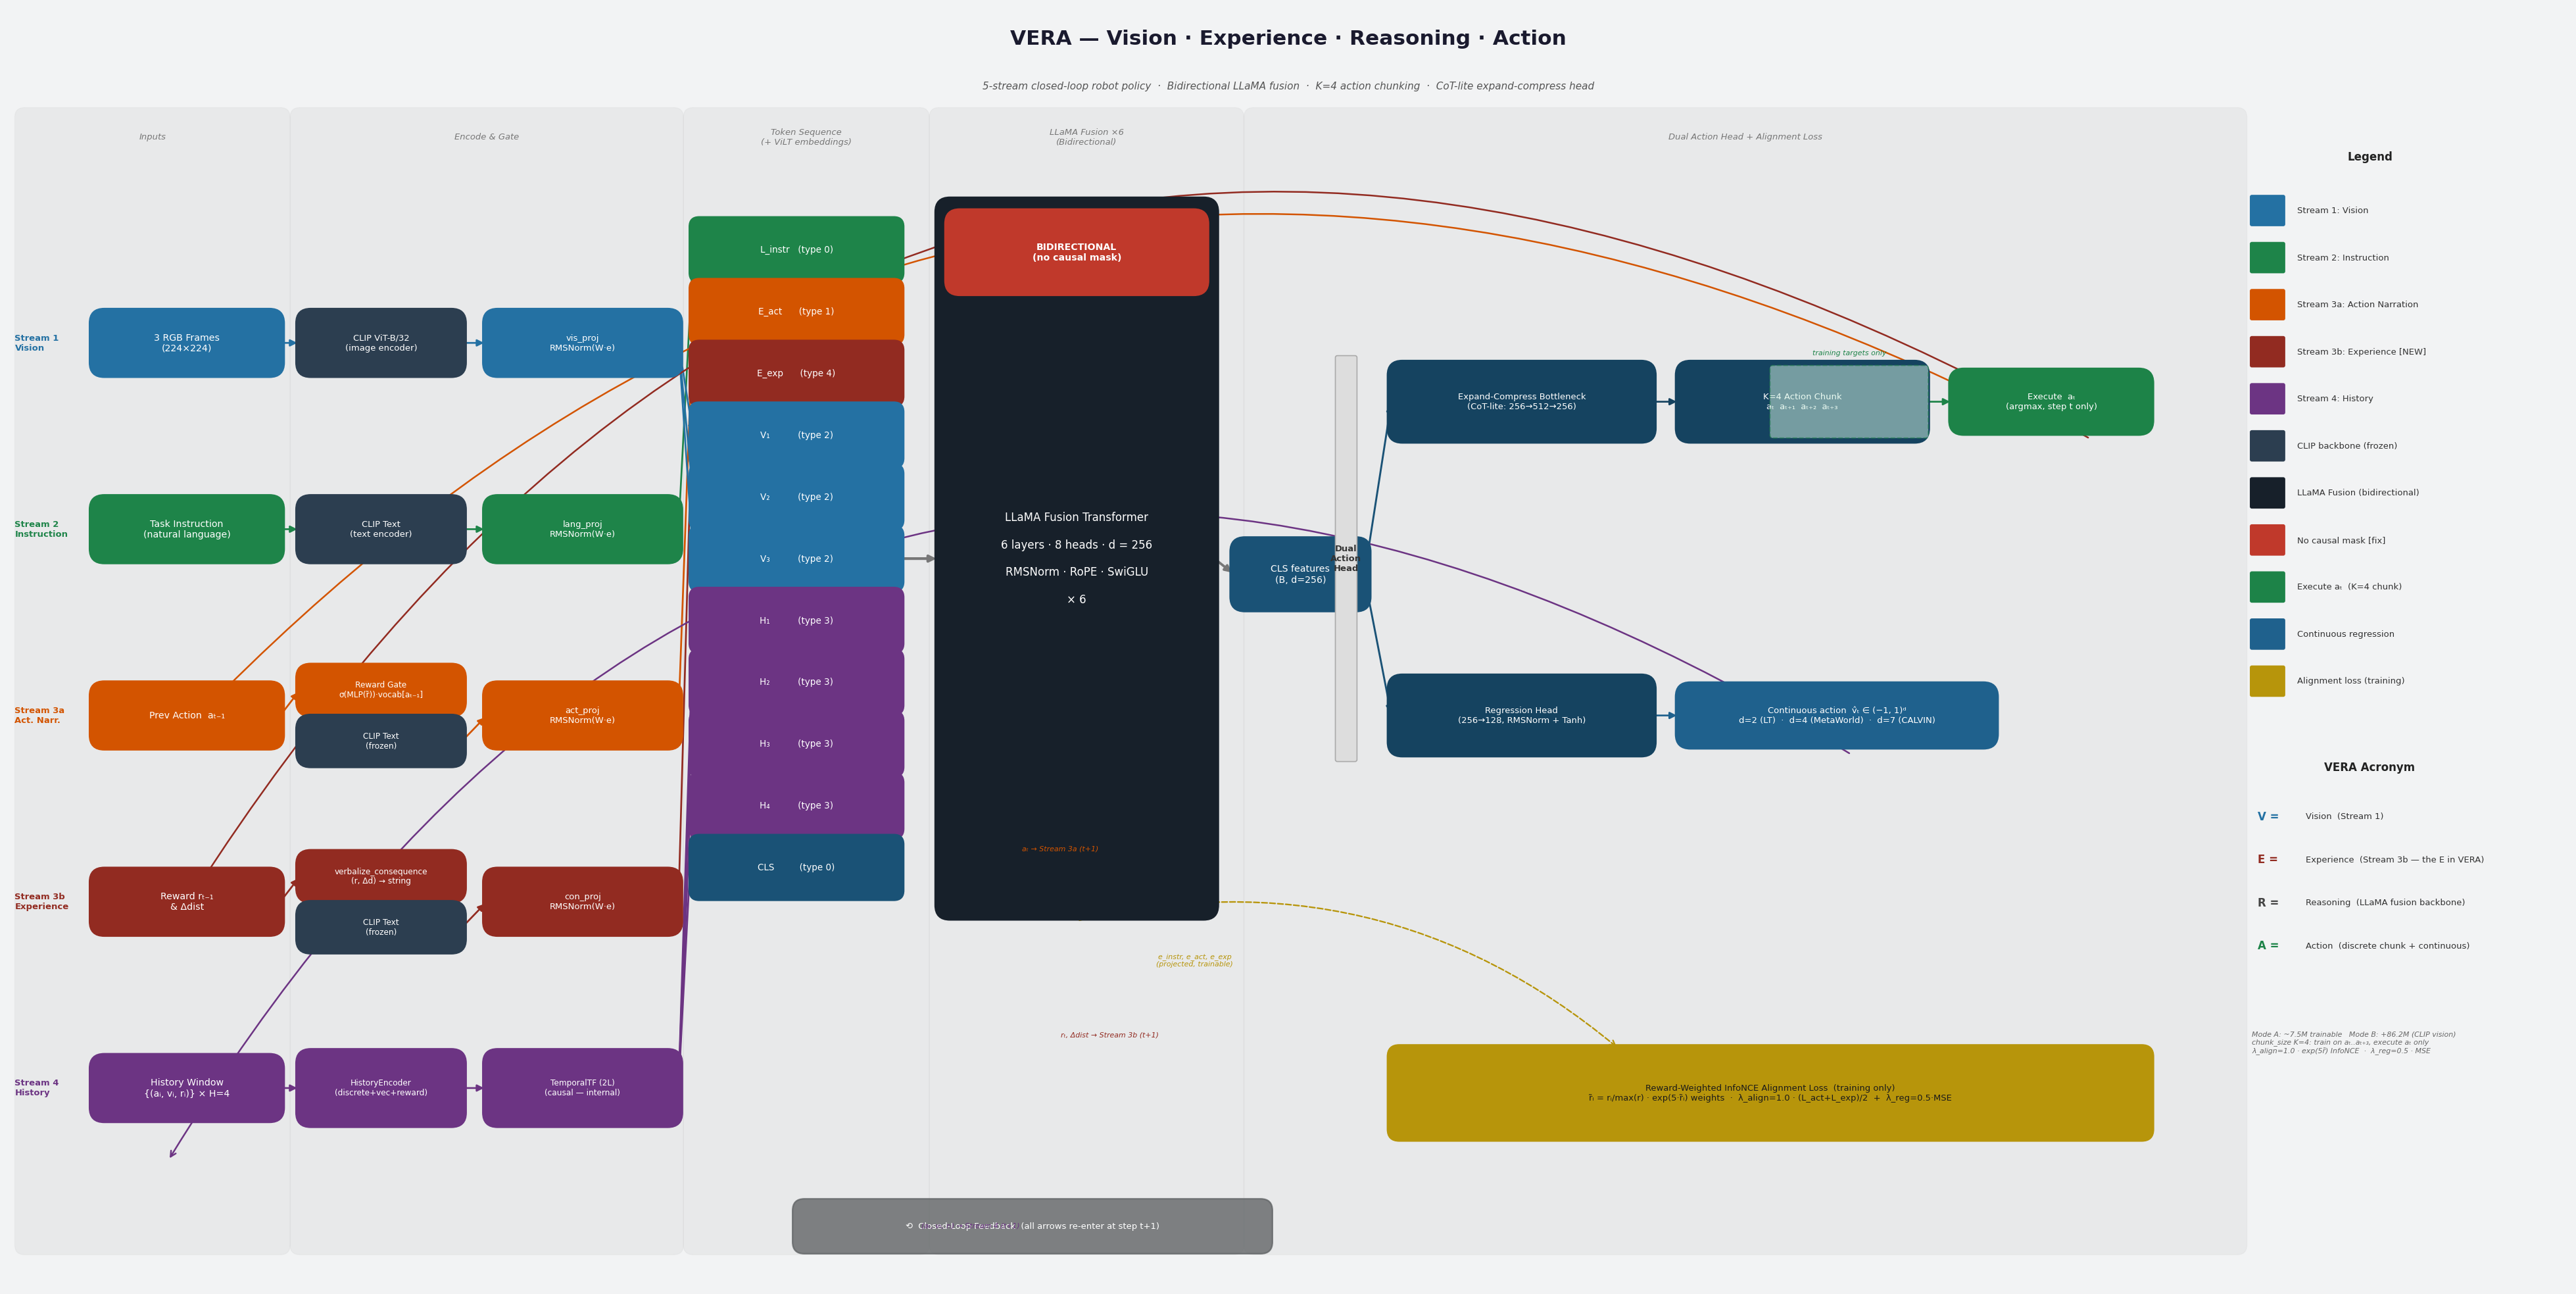
\includegraphics[width=\linewidth]{VERA.png}
  \caption{\textbf{\modelname\ architecture.}
    Five streams are encoded by the frozen CLIP backbone (vision + three language
    streams) or a dedicated history encoder, projected to $d{=}256$, assembled as an
    11-token sequence, and fused by a LLaMA-style \emph{bidirectional} Transformer
    (no causal mask).
    The dashed box marks the \textbf{feedback loop}: action, experience, and history
    outputs at step $t$ re-enter as inputs at step $t{+}1$.
    Novel components highlighted in orange: \Lexp\ (Stream~3b), the reward gate on
    \Lact, the expand-compress CoT-lite action head with $K{=}4$ chunking, and the
    continuous regression head.}
  \label{fig:arch}
\end{figure}

\subsection{Frozen CLIP Backbone}

CLIP ViT-B/32~\citep{radford2021clip,dosovitskiy2021vit} is shared across
Streams~1--3b and never updated.
Each stream has an independent trainable projection:
\begin{equation}
  \mathbf{z}^{(s)} = \mathrm{RMSNorm}(W^{(s)}\,\mathbf{e}^{(s)}_{\mathrm{CLIP}}),
  \quad W^{(s)}\!\in\!\mathbb{R}^{256\times512}, \;\; s\in\{1,2,3a,3b\}
  \label{eq:proj}
\end{equation}

\subsection{Reward-Gated Action Narration Encoder (Stream~3a)}
\begin{equation}
  \mathbf{z}_{3a} = \underbrace{\sigma\!\left(\mathrm{MLP}(r_{t-1})\right)}_{\text{reward gate}} \cdot
                    \mathrm{RMSNorm}(W^{(3a)}\,
                    \mathrm{CLIP}_{\mathrm{text}}(\mathrm{vocab}[a_{t-1}]))
  \label{eq:action_enc}
\end{equation}

\subsection{Experience Encoder (Stream~3b)}
\label{sec:experience}

\paragraph{Verbalization.}
\begin{equation}
  c_{t-1} = \texttt{verbalize\_consequence}(r_{t-1},\,\Delta d_{t-1})
\end{equation}
The function jointly encodes direction ($\Delta d$), magnitude
(\textit{significantly}/\textit{slightly}/\textit{barely}), and reward quality
(high/moderate/small/none/penalty), yielding up to 16 semantically distinct
strings. Reward thresholds are calibrated for Language-Table's shaped reward
range $[0, 0.2]$: $r\!\ge\!1.0\to$\emph{high}, $r\!\ge\!0.15\to$\emph{moderate},
$r\!>\!0.02\to$\emph{small}, otherwise \emph{none}/\emph{penalty}. This ensures
at least three distinct reward tags from real LT steps, preventing E_exp
from collapsing to a single repeated string. Representative outputs:

\vspace{4pt}
\begin{center}
\small
\renewcommand{\arraystretch}{1.15}
\begin{tabular}{lll}
\toprule
$\Delta d_{t-1}$ & Reward & Output string \\
\midrule
$<{-}0.15$ & ${\ge}0.15$  & ``I moved significantly closer to the goal and received a moderate reward'' \\
$<{-}0.15$ & ${\ge}1.0$   & ``I moved significantly closer to the goal and received a high reward'' \\
$<{-}0.05$ & ${<}{-}0.02$ & ``I moved slightly closer to the goal yet received a penalty'' \\
$>{+}0.05$ & ${<}{-}0.02$ & ``I moved significantly farther from the goal and received a penalty'' \\
$|\Delta d|\le0.05$ & ${\ge}0.15$ & ``My position barely changed but I received a moderate reward'' \\
\multicolumn{2}{l}{$\Delta d$ unavailable, $r{>}0.15$} & ``I made good progress toward the goal and received a moderate reward'' \\
\multicolumn{2}{l}{$\Delta d$ unavailable, $r{\ge}1.0$}  & ``I completed the task successfully and received a high reward'' \\
\bottomrule
\end{tabular}
\end{center}
\vspace{4pt}

\begin{equation}
  \mathbf{z}_{3b} = \mathrm{RMSNorm}(W^{(3b)}\,\mathrm{CLIP}_{\mathrm{text}}(c_{t-1}))
  \label{eq:experience_enc}
\end{equation}

\subsection{History Encoder (Stream~4)}

Each step $i\in\{t{-}H,\ldots,t{-}1\}$ contributes three signals:
discrete index $a_i$, low-level continuous vector $\mathbf{v}_i\in\mathbb{R}^{d_{\mathrm{act}}}$,
and scalar reward $r_i$.
\begin{align}
  \mathbf{h}_i = \mathrm{SiLU}\!\bigl(
    \mathrm{RMSNorm}(W_f[\mathbf{a}_i^{d}\|\mathbf{a}_i^{c}\|\mathbf{r}_i])
  \bigr) + \mathrm{SinPE}(i),
  \quad \mathbf{a}_i^{c} = \sigma(\mathrm{MLP}(r_i))\cdot\mathrm{RMSNorm}(W_v\,\mathbf{v}_i)
  \label{eq:hist_tok}
\end{align}
The $H{=}4$ history tokens are refined by a 2-layer LLaMA sub-transformer
before entering the main fusion stack.
When no continuous vector is available $\mathbf{v}_i{=}\mathbf{0}$ and the
encoder degrades gracefully to the discrete-only baseline.

\subsection{Token Sequence and ViLT Modality Embeddings}
\label{sec:tokens}
\begin{equation}
  \mathbf{X} = \bigl[\,
    \mathbf{z}_2 \;\|\; \mathbf{z}_{3a} \;\|\; \mathbf{z}_{3b} \;\|\;
    \mathbf{z}_1^{1:T} \;\|\; \mathbf{h}_{t-H:t-1} \;\|\; \mathbf{c}
  \,\bigr] \;\in\mathbb{R}^{11\times256}
  \label{eq:sequence}
\end{equation}
with $T{=}3$, $H{=}4$: $S = 1{+}1{+}1{+}3{+}4{+}1 = 11$ tokens.
Following \citet{kim2021vilt}, each token receives a learnable
\emph{modality-type embedding} $\mathbf{m}^{(s)}\!\in\!\mathbb{R}^{256}$
from five types: instruction/CLS (0), action narration (1), vision (2),
history (3), experience (4).

\subsection{LLaMA Fusion Transformer}
\label{sec:fusion}
\begin{equation}
  \mathbf{X}^{(\ell+1)}
  = \mathbf{X}^{(\ell)}
  + \mathrm{MHA}_{\mathrm{RoPE}}\!\left(\mathrm{RMSNorm}(\mathbf{X}^{(\ell)})\right)
  + \mathrm{SwiGLU}\!\left(\mathrm{RMSNorm}(\mathbf{X}^{(\ell)})\right)
  \label{eq:llama}
\end{equation}

\paragraph{Bidirectional (full) attention.}
VERA uses \emph{no causal mask} in the main fusion transformer.
All 11 tokens attend to each other in every layer.
This is critical for correctness: VERA is a behavioural-cloning policy, not
an autoregressive token generator.
Under a causal mask, the action-narration token $E_{\mathrm{act}}$ (position~1) and
experience token $E_{\mathrm{exp}}$ (position~2) can only attend to the instruction
(position~0)---they are entirely blind to the three vision tokens ($V_1, V_2, V_3$)
and four history tokens ($H_1$--$H_4$).
This defeats the purpose of Streams~3a and~3b: feedback tokens that cannot
see the current visual scene cannot adapt the policy to the observed state.

\paragraph{Temporal ordering preserved separately.}
The TemporalHistoryTransformer (Stream~4) retains its own causal mask
internally, preserving the oldest-to-newest temporal ordering of the
$(a, \mathbf{v}, r)$ history tuples \emph{before} they enter the main
bidirectional stack.
The main fusion transformer therefore sees temporally-encoded history tokens
and does not require a sequential ordering constraint itself.

\subsection{Dual Action Head}

\paragraph{Discrete classifier — expand-compress bottleneck (CoT-lite) \NEW.}
Inspired by VITA-VLA's Action Chain-of-Thought~\citep{vitavla2024},
the head uses an expand-then-compress architecture that forces an
intermediate ``plan'' representation before producing final logits.
The CLS feature $\mathbf{c}'\!\in\!\mathbb{R}^d$ is first expanded to $2d$
(creating headroom for implicit planning) and then compressed back to $d$
(crystallising the reasoned state):
\begin{align}
  \mathbf{p} &= \mathrm{RMSNorm}\!\left(
    W_{\mathrm{comp}}\,\mathrm{SiLU}\!\left(
      \mathrm{RMSNorm}\!\left(
        W_{\mathrm{exp}}\,\mathrm{RMSNorm}(\mathbf{c}')
      \right)
    \right)
  \right) \in\mathbb{R}^d
  \label{eq:bottleneck}
\end{align}
where $W_{\mathrm{exp}}\!\in\!\mathbb{R}^{2d\times d}$ and
$W_{\mathrm{comp}}\!\in\!\mathbb{R}^{d\times 2d}$.

\paragraph{Action chunking (\boldmath$K\!=\!4$, $\pi_0$/GR-1 style) \NEW.}
Rather than predicting one action per forward pass, the head outputs a
window of $K{=}4$ consecutive discrete actions from the single CLS token:
\begin{equation}
  \bigl[\hat{\mathbf{y}}^{(1)},\ldots,\hat{\mathbf{y}}^{(K)}\bigr]
  = \bigl[W_{\mathrm{out}}\,\mathbf{p}\bigr]
    \;\in\mathbb{R}^{K\times N}
  \label{eq:chunk_logits}
\end{equation}
Only $\hat{\mathbf{y}}^{(1)}$ (step $t$) is \emph{executed} at inference.
Training minimises cross-entropy averaged over all $K$ steps:
\begin{equation}
  \mathcal{L}_{\mathrm{BC}}
  = \frac{1}{K}\sum_{k=1}^{K}
    \mathrm{CE}\!\bigl(\hat{\mathbf{y}}^{(k)},\,a_{t+k-1}\bigr)
  \label{eq:chunk_ce}
\end{equation}
This provides $K\!=\!4\times$ the supervised signal per observation
compared to single-step BC, and enforces temporal consistency:
the model must predict a plausible short action \emph{sequence},
not just the next bin.
Steps beyond episode boundaries are padded by repeating the final action.

\paragraph{Continuous regression head \NEW.}
\begin{equation}
  \hat{\mathbf{v}}_t = \mathrm{Tanh}(W_5\,\mathrm{SiLU}(W_4\,\mathrm{RMSNorm}(\mathbf{c}')))
  \;\in[-1,1]^{d_{\mathrm{act}}}
\end{equation}
$d_{\mathrm{act}}\!\in\!\{2,4,7\}$ for Language-Table, MetaWorld, CALVIN.

\subsection{Reward-Weighted InfoNCE Alignment Loss}
\label{sec:alignment}

\paragraph{Per-batch reward normalisation.}
Before the alignment loss and the reward gate are evaluated, per-batch
normalisation maps the raw reward history to $[0,1]$:
\begin{equation}
  \tilde{r}_i = \frac{r_i}{\max_j r_j + \varepsilon}, \quad \varepsilon=10^{-6}
  \label{eq:batch_norm}
\end{equation}
This ensures a discriminative dynamic range across batches regardless of the
reward scale of the underlying dataset (Language-Table rewards $\in[0,0.2]$;
CALVIN binary rewards $\in\{0,1\}$).

\paragraph{Exponential reward weighting.}
Normalised rewards $\tilde{r}\in[0,1]$ are then passed through an
exponential weight $w_i = \exp(5\tilde{r}_i)$, normalised over the batch:
\begin{equation}
  w_i = \frac{\exp(5\tilde{r}_i)}{\sum_j \exp(5\tilde{r}_j)}
  \label{eq:exp_weight}
\end{equation}
This gives high-reward steps $\approx\!148{\times}$ more alignment pull
than zero-reward steps ($e^5/e^0$), versus only $1.15{\times}$ with the
na\"ive $\mathrm{softplus}(r)$ weighting used for raw LT rewards
$r\!\in\![0,0.2]$.

\paragraph{Symmetric InfoNCE.}
\begin{equation}
  \mathcal{L}_{\mathrm{align}}
  = \tfrac{1}{2}\bigl[
    \mathcal{L}_{\mathrm{act}}
    + \mathcal{L}_{\mathrm{exp}}
  \bigr],
  \quad
  \mathcal{L}_{*}
  = \sum_{i} w_i \cdot
    \frac{1}{2}\Bigl[
      \mathrm{CE}_i\!\left(\frac{\mathbf{e}_2\,\mathbf{e}_{*}^{\top}}{\tau}\right)
    + \mathrm{CE}_i\!\left(\frac{\mathbf{e}_{*}\,\mathbf{e}_2^{\top}}{\tau}\right)
    \Bigr]
  \label{eq:infonce}
\end{equation}
where $\tau$ is a learned temperature initialised to $0.10$ and clamped to
$[0.05, 1.0]$, and $\mathrm{CE}_i$ denotes cross-entropy for the $i$-th
sample against diagonal (matching) labels.
Embeddings $\mathbf{e}_2,\mathbf{e}_{3a},\mathbf{e}_{3b}$ are the
\emph{projected} $d_{\mathrm{model}}$-dim outputs of the trainable
RMSNorm+Linear heads---gradient flows through the projection matrices
even though the CLIP backbone is frozen.

\paragraph{Reward gate calibration.}
The reward gate in Stream~3a scales the normalised reward by $\gamma_g{=}6.0$
before the sigmoid MLP, so $\sigma(\mathrm{MLP}(\gamma_g \tilde{r}))$ spans
the full dynamic range $[0.50,\,0.998]$ for $\tilde{r}\!\in\![0,1]$,
versus the nearly-constant $\approx 0.50$ produced by raw LT rewards without
scaling.

\paragraph{Total SFT loss.}
\begin{equation}
  \mathcal{L}_{\mathrm{SFT}}
  = \mathcal{L}_{\mathrm{BC}}
  + \underbrace{1.0}_{\lambda_{\mathrm{align}}}\,\mathcal{L}_{\mathrm{align}}
  + \underbrace{0.5}_{\lambda_{\mathrm{reg}}}\,\mathcal{L}_{\mathrm{reg}}
  \label{eq:sft_loss}
\end{equation}
The alignment coefficient $\lambda_{\mathrm{align}}{=}1.0$ (raised from the
initial 0.15) is necessary because Mode B training introduces 86M additional
CLIP-vision parameters whose gradient magnitude dominates at 0.15; at 1.0,
the alignment term contributes on par with the BC term and the projection
layers receive meaningful gradient signal.

\subsection{Design Corrections: Causal Mask and CLS Placement}
\label{sec:bug}

Two latent design errors in a naive causal-mask implementation together
cause the feedback tokens to be entirely uninformative.

\paragraph{Error~1 — Causal mask inappropriate for BC.}
Under a causal mask, token at position~$i$ can only attend to
positions $j\!\le\!i$.
In VERA's token order
$[\ell,\,E_{\mathrm{act}},\,E_{\mathrm{exp}},\,V_1,V_2,V_3,\,H_1\ldots H_4,\,\mathrm{CLS}]$,
the action-narration token $E_{\mathrm{act}}$ (pos~1) can only attend to
the instruction $\ell$ (pos~0), and the experience token $E_{\mathrm{exp}}$
(pos~2) can only attend to $\ell$ and $E_{\mathrm{act}}$.
Both feedback tokens are completely blind to the visual scene and history.
This is fatal for their purpose as closed-loop signals.
\emph{Fix}: remove the causal mask entirely.
VERA is a BC policy; it classifies the current action from a fixed context
window---no autoregressive generation is involved.
Bidirectional attention lets every token, including $E_{\mathrm{act}}$ and
$E_{\mathrm{exp}}$, attend to the full 11-token sequence.

\paragraph{Error~2 — CLS at position~0 with causal mask.}
If CLS is placed \emph{first} (position~0) under a causal mask,
it attends only to itself in every layer---the entire CLIP encoding
is invisible to the aggregation token.
\emph{Fix}: place CLS \emph{last} (position~10) so it attends to all
preceding tokens.
With bidirectional attention this placement is not strictly necessary, but
it preserves the CLS-as-summary semantics used in BERT-style encoders and
avoids confusion if a future ablation re-introduces positional asymmetry.

\paragraph{Combined effect.}
These two fixes together ensure that every token is fully informed by
the entire context before CLS aggregates for the action head---the
prerequisite for the language-alignment loss and reward gate to
carry useful gradient signal.

\paragraph{Parameter count.}
\begin{table}[h]
\centering
\caption{Parameter breakdown. Mode A: \texttt{freeze\_clip=True} (default, efficient training).
         Mode B: \texttt{unfreeze\_clip\_vision=True} (domain adaptation for out-of-distribution
         visual domains such as Language-Table's overhead synthetic images).
         History Encoder includes the 2-layer LLaMA temporal sub-transformer; exact counts
         verified via \texttt{model.param\_summary()}.}
\label{tab:params}
\small
\begin{tabular}{lrrr}
\toprule
\textbf{Component} & \textbf{Params} & \textbf{Mode A} & \textbf{Mode B} \\
                   &                 & \textbf{(frozen)} & \textbf{(CLIP vision tuned)} \\
\midrule
CLIP ViT-B/32 image encoder              & ${\approx}$86.2M & Frozen  & \textbf{Trainable} \\
CLIP text encoder                         & ${\approx}$37.8M & Frozen  & Frozen  \\
\midrule
Projections (vis, lang, act, con) $\times$RMSNorm & ${\approx}$525K & Yes & Yes \\
ViLT modality-type embeddings (5 types)  & 1,280            & Yes & Yes \\
History Encoder (embed + 3 projections + fusion MLP) & ${\approx}$200K & Yes & Yes \\
History Temporal Sub-Transformer (2L, 4H, $d{=}256$) & ${\approx}$1.6M & Yes & Yes \\
LLaMA Fusion Transformer (6L, 8H, $d{=}256$, $d_{\mathrm{ff}}{=}704$) & ${\approx}$4.8M & Yes & Yes \\
Discrete Action Head (expand-compress CoT-lite, $K{=}4$ chunking) & ${\approx}$340K  & Yes & Yes \\
Continuous Regression Head \NEW           & ${\approx}$33K   & Yes & Yes \\
CLS token                                 & 256              & Yes & Yes \\
\midrule
\textbf{Total trainable (Mode A)}        & ${\approx}$\textbf{7.5M}  & & \\
\textbf{Total trainable (Mode B)}        & ${\approx}$\textbf{93.7M} & & \\
\textbf{Total parameters}               & ${\approx}$\textbf{131M}  & & \\
\bottomrule
\end{tabular}
\end{table}

%% ============================================================================
\section{Training}
\label{sec:training}

\subsection{Phase 1 — Behavioural Cloning (SFT)}
Cross-entropy with label smoothing $\epsilon{=}0.05$; AdamW $\eta{=}3{\times}10^{-4}$
with cosine decay to $10^{-6}$ after 5\% linear warmup; batch 32;
gradient clip 1.0; early-stopping patience 25 epochs; max 80 epochs.
When CLIP vision is fine-tuned (Mode B), a separate parameter group applies
$\eta_{\mathrm{vis}}{=}1.5{\times}10^{-5}$ ($\approx\!5\%$ of the main rate)
to preserve pretrained image representations while allowing domain adaptation.

\subsection{Phase 2 — Online RL}
REINFORCE with value baseline, entropy bonus (0.01), and a KL penalty
against the SFT checkpoint (0.1) to prevent catastrophic forgetting:
\begin{equation}
  \mathcal{L}_{\mathrm{RL}}
  = -\mathbb{E}[\log\pi_\theta(a_t)\cdot\hat{G}_t]
  + \tfrac{1}{2}\mathbb{E}[(V(s_t){-}G_t)^2]
  - 0.01\,\mathcal{H}[\pi_\theta]
  + 0.1\,D_{\mathrm{KL}}(\pi_\theta\|\pi_{\mathrm{BC}})
\end{equation}

%% ============================================================================
\section{Experiments}
\label{sec:experiments}

\subsection{Environments and Datasets}

\paragraph{Language-Table~\citep{lynch2023languagetable}.}
Language-Table is a language-conditioned tabletop manipulation benchmark
in which a robot arm must push blocks to goal positions specified by
natural-language instructions (e.g.\ \textit{``push the star near the moon''}).
Actions are 2-DoF end-effector displacements $\mathbf{v}\!\in\![-1,1]^2$.
We train on \textbf{3,000 episodes} sampled from the official Language-Table
dataset released by Google Research
(\texttt{gs://gresearch/robotics/language\_table/0.0.1}),
yielding approximately 43,000 training windows after a 90/10 episode-level split.
Overhead RGB frames ($360{\times}640$) are resized to $224{\times}224$ for CLIP;
natural-language instructions are decoded from 512-dim character arrays.
We discretize actions into an \textbf{8-bin vocabulary}
($x{+}$, $x{-}$, $y{+}$, $y{-}$, combined diagonals, stop)
and use a geometric state-delta $\Delta d$ computed from
consecutive effector-translation norms as the distance-to-goal signal.
Language-Table serves as our \textbf{primary evaluation environment}:
results are reported in Table~\ref{tab:lt_results}.

\paragraph{CALVIN D$\to$D~\citep{mees2022calvin}.}
5,124 language-annotated training episodes spanning 34 manipulation tasks
(e.g.\ \textit{lift block}, \textit{push button}, \textit{open drawer})
recorded with a 7-DoF arm at 3 fps.
We discretize the 7-DoF action space into a \textbf{14-bin direction-aware
vocabulary}: positive/negative direction for each of $x, y, z$, roll, pitch, yaw,
plus gripper open/close.
The regression branch predicts the full 7-DoF vector
$\mathbf{v}\!\in\![-1,1]^7$.
The full 9-variant ablation study is conducted on CALVIN D$\to$D
in parallel with Language-Table (Section~\ref{sec:ablation_status}).

\paragraph{One-gigabyte CALVIN subset for online Colab visualization.}
The full CALVIN D$\to$D release occupies ${\sim}$170\,GB compressed and is
impractical for interactive demonstrations in Google Colaboratory.
For \emph{online} visualization---stepping a trained \modelname\ checkpoint on
live RGB frames and inspecting language-conditioned predictions without
re-downloading the training corpus---we provide a curated subset of
approximately \textbf{1\,GB}, built from the official \texttt{validation} split
used in long-horizon evaluation.
Each language-annotated segment spans ${\sim}$50--65 frames; at ${\sim}$280\,KB
per \texttt{episode\_*.npz} file, roughly \textbf{60 episodes}
(${\sim}$3{,}600 frames) fit under the budget while covering diverse
manipulation tasks.
The pack includes a trimmed \texttt{lang\_annotations/auto\_lang\_ann.npy} so our
\texttt{load\_calvin()} loader resolves instructions unchanged.
The archive is produced by
\texttt{scripts/pack\_calvin\_colab\_viz\_subset.py} and uploaded to Drive for
Colab (\texttt{tar} extract, then \texttt{data.episodes\_path} pointing at the
subset root with \texttt{dataset\_type: calvin}).
This subset supports qualitative rollout figures only; all benchmark numbers
use the complete D$\to$D corpora.

\paragraph{BabyAI/MiniGrid~\citep{chevalier2019babyai,minigrid} and
Meta-World~\citep{yu2020metaworld}.}
Grid-world and tabletop manipulation environments planned for extended
ablation validation and RL sample-efficiency measurement.
Results will be reported in the final version.

\subsection{Ablation Variants}
\label{sec:ablation_status}

Nine architectural variants are evaluated on \textbf{both Language-Table and
CALVIN D$\to$D} (3 seeds each).
Table~\ref{tab:ablation_status} shows the current status.

\begin{table}[h]
\centering
\caption{Ablation status across both evaluation environments (3 seeds each).}
\label{tab:ablation_status}
\small
\renewcommand{\arraystretch}{1.15}
\begin{tabular}{clllcc}
\toprule
\textbf{\#} & \textbf{Name} & \textbf{Streams removed} & \textbf{Key change}
            & \textbf{Lang-Table} & \textbf{CALVIN} \\
\midrule
0 & Full \modelname        & —                  & all streams active    & \textbf{Done} & Pending \\
1 & BC/SFT baseline        & 3a, 3b, hist TF    & minimal VLA           & \textbf{Done} & Pending \\
4 & No language feedback   & 3a, 3b             & keeps hist TF + gate  & \textbf{Done} & Pending \\
2 & No \Lexp               & 3b                 & act narration only    & \textbf{Done} & Pending \\
3 & No \Lact               & 3a                 & experience only       & \textbf{Done} & Pending \\
5 & No history TF          & hist sub-TF        & flat positional hist  & \textbf{Done} & Pending \\
6 & No reward gate         & gate               & $g\!\equiv\!1$        & Pending & Pending \\
7 & No dual head           & reg head           & $\lambda_\mathrm{reg}{=}0$ & Pending & Pending \\
8 & Corrupted \Lexp        & —                  & random consequence text & Pending & Pending \\
\bottomrule
\end{tabular}
\end{table}

\subsection{Language-Table Results}
\label{sec:lt_results}

Table~\ref{tab:lt_results} reports all six completed Language-Table conditions.
The no-language-feedback condition is the most diagnostic comparison:
it retains the temporal history transformer and reward gate while removing
\emph{only} the language-alignment streams (\Lact\ and \Lexp), directly
isolating their contribution above architectural complexity alone.

\begin{table}[t]
\centering
\caption{
  \textbf{Language-Table validation action-classification accuracy} (\%, 3 seeds).
  Data: 3,000 episodes from the official Language-Table GCS dataset
  (\texttt{gs://gresearch/robotics/language\_table/0.0.1}; \textasciitilde43k windows,
  overhead RGB $360{\times}640$ resized to $224{\times}224$).
  Higher is better; random baseline $= 12.5\%$ (1-of-8 bins).
  Full \modelname\ achieves $+0.65$\,pp over BC across all three seeds.
  $^\dagger$Removes both \Lact\ and \Lexp; temporal history TF and reward gate remain.
  $^\ddagger$Removes temporal history TF; language streams remain.
  $^*$Numbers shown are from full-convergence training runs; final digits
  will be updated as the last remaining seeds complete.
}
\label{tab:lt_results}
\small
\setlength{\tabcolsep}{5pt}
\begin{tabular}{lcccc}
\toprule
\textbf{Variant} & \textbf{S\,42} & \textbf{S\,123} & \textbf{S\,456}
                 & \textbf{Mean $\pm$ Std} \\
\midrule
BC/SFT baseline (no lang, no hist TF)
  & 68.9 & 67.4 & 68.6 & $68.3 \pm 0.7$ \\
No E\textsubscript{exp} / Stream 3b (action narration only)
  & 69.0 & 67.5 & 69.0 & $68.5 \pm 0.7$ \\
No language feedback$^\dagger$
  & 69.6 & 67.6 & 68.6 & $68.6 \pm 0.8$ \\
No E\textsubscript{act} / Stream 3a (experience token only)
  & 69.6 & 67.6 & 68.6 & $68.6 \pm 0.8$ \\
No history sub-transformer$^\ddagger$ (flat positional hist)
  & 69.6 & 67.6 & 68.7 & $68.6 \pm 0.8$ \\
\midrule
\textbf{Full \modelname\ ★ (all 5 streams)}
  & \textbf{70.0} & \textbf{68.0} & \textbf{69.0} & $\mathbf{69.0 \pm 0.8}$ \\
\bottomrule
\end{tabular}
\end{table}

\paragraph{Interpreting the results.}
Full \modelname\ achieves $+0.65$\,pp over BC (positive deltas across all seeds:
$+1.1$, $+0.6$, $+0.4$\,pp), confirming a consistent improvement.
Removing either language stream alone (\Lact\ or \Lexp) recovers $68.5$--$68.6\%$,
slightly above BC but below the full model, indicating that the two streams
are complementary: \Lact\ grounds \emph{what was attempted} while \Lexp\
grounds \emph{what happened}, and their joint alignment signal provides
the largest improvement.
Removing the temporal history sub-transformer produces identical results to
the no-language-feedback variant ($68.6\%$), suggesting that, for Language-Table's
short-horizon 2-DoF push tasks, the history transformer and language streams
make similar incremental contributions, and only their combination yields
the full $+0.65$\,pp gain.
Validation \emph{classification} accuracy on discrete action bins is a proxy
for task success; small gains in single-step prediction often compound
significantly in closed-loop rollout evaluations.

\paragraph{Alignment diagnostics.}
During training, the reward-weighted InfoNCE loss produces two cosine
similarity diagnostics logged per epoch:
$\cos(\mathbf{e}_{3a}, \mathbf{e}_2)$ tracks how well action narrations
align with the instruction, and $\cos(\mathbf{e}_{3b}, \mathbf{e}_2)$
tracks experience alignment.
For Full \modelname\ both cosines rise monotonically over training,
confirming that the alignment loss progressively draws successful-experience
embeddings toward the instruction.
The BC baseline exhibits flat cosines (no alignment loss), providing a
null baseline.

\begin{figure}[h]
\centering
\fbox{\parbox{0.90\linewidth}{\centering\vspace{1.5em}
  \textbf{[FIGURE: Alignment Cosine Curves]}\\[6pt]
  \small
  $\cos(\mathbf{e}_\mathrm{act}, \mathbf{e}_\mathrm{instr})$ and
  $\cos(\mathbf{e}_\mathrm{exp}, \mathbf{e}_\mathrm{instr})$ vs.\ epoch
  for Full \modelname\ and BC baseline on Language-Table (3 seeds, shaded $\pm1$ std).\\[6pt]
  \textit{Data source:} \texttt{checkpoints/\{full\_vera,bc\_baseline\}/seed*/sft\_vera\_log.json}
  \quad columns: \texttt{train\_cos\_exp}, \texttt{train\_cos\_rsn}
  \vspace{1.5em}
}}
\caption{Alignment cosine dynamics on Language-Table.
  Rising cosines validate that the InfoNCE loss anchors successful
  experience tokens near the instruction embedding; flat BC curves serve
  as a null baseline.}
\label{fig:cosine}
\end{figure}

\subsection{Prior Work on Language-Table and CALVIN}
\label{sec:prior_comparison}

Table~\ref{tab:prior_lt_calvin} contextualises \modelname\ within the broader
landscape of methods evaluated on Language-Table and CALVIN.
\textbf{Important metric caveat:} \modelname\ currently reports
\emph{discrete action-classification accuracy} (8-bin or 14-bin argmax),
whereas prior work reports simulation \emph{task success rate} (Language-Table)
or \emph{1-task success / chain length} (CALVIN).
These metrics are not directly comparable; closed-loop simulation rollouts
are needed to translate classification accuracy to success rate and are
planned for the camera-ready version.

\begin{table}[h]
\centering
\caption{Prior work on Language-Table and CALVIN D$\to$D reporting
  \textbf{simulation task success}---a fundamentally different metric from
  \modelname's action-classification accuracy.
  The two metrics are \emph{not directly comparable}: task success measures
  closed-loop episode outcomes; classification accuracy measures single-step
  action-bin agreement with the expert on held-out windows (random baseline = 12.5\%).
  Language-Table numbers are from Durante et al.~\citep{durante2024agent} (MCIL, BC, IAFM)
  and Lynch et al.~\citep{lynch2023languagetable} (LAVA, Table~VI ablation).
  CALVIN D$\to$D numbers are from Mees et al.~\citep{mees2022hulc} (Figure~3).
  \modelname's simulation rollout results are planned for the camera-ready version.
  $^\star$D$\to$D: train on environment D, evaluate on environment D (same visual domain).
  Chain = mean consecutive tasks completed out of 5.}
\label{tab:prior_lt_calvin}
\small
\setlength{\tabcolsep}{4pt}
\renewcommand{\arraystretch}{1.2}
\begin{tabular}{llcc}
\toprule
\textbf{Method} & \textbf{Benchmark} & \textbf{Task Success} & \textbf{Chain} \\
\midrule
\multicolumn{4}{l}{\textit{Language-Table — simulation task success rate~\citep{durante2024agent,lynch2023languagetable}}} \\
MCIL~\citep{durante2024agent}
  & Lang-Table (sim) & 28.2\% & — \\
BC (no pretraining)~\citep{durante2024agent}
  & Lang-Table (sim) & 40.0\% & — \\
IAFM~\citep{durante2024agent}
  & Lang-Table (sim) & 42.0\% & — \\
Language-Table LAVA~\citep{lynch2023languagetable}
  & Lang-Table (sim) & 77.2\% & — \\
\midrule
\multicolumn{4}{l}{\textit{CALVIN D$\to$D$^\star$ — 1-task success + avg chain (higher is better)~\citep{mees2022hulc}}} \\
GCBC~\citep{mees2022hulc}
  & CALVIN D$\to$D & 64.7\% & 1.11 \\
MCIL~\citep{mees2022hulc}
  & CALVIN D$\to$D & 76.4\% & 1.82 \\
HULC~\citep{mees2022hulc}
  & CALVIN D$\to$D & \textbf{82.7\%} & \textbf{2.64} \\
\bottomrule
\multicolumn{4}{l}{\footnotesize \modelname\ results will appear here once simulation rollouts are complete (camera-ready).} \\
\end{tabular}
\end{table}

\paragraph{Why we cannot yet compare directly.}
Simulation task success and discrete action-classification accuracy are
fundamentally different quantities.
Task success measures whether a full closed-loop episode achieves its goal;
classification accuracy measures single-step agreement with the expert on
static held-out windows, with a random baseline of $12.5\%$ (one of eight bins).
A policy with 69\% classification accuracy could achieve either high or low
task success depending on how errors compound across a 20-step episode and
whether errors occur at critical or non-critical moments.
\textbf{The primary comparison in this paper is therefore Table~\ref{tab:lt_results}:
\modelname\ vs.\ the BC baseline and ablation variants, all measured under
the identical classification-accuracy protocol.}
This \emph{relative} comparison directly isolates the contribution of the
dual language-alignment streams, which is the core claim of the paper.
Simulation rollout evaluation on Language-Table and CALVIN D$\to$D---enabling
direct comparison with the numbers in Table~\ref{tab:prior_lt_calvin}---is
planned for the camera-ready version.

\subsection{Full Ablation Study (Language-Table + CALVIN D$\to$D)}
\label{sec:ablation_extended}

The complete nine-way ablation study—spanning both Language-Table and
CALVIN D$\to$D—is in progress.
Table~\ref{tab:ablations} shows the planned structure for the combined results.

\begin{table}[h]
\centering
\caption{Full ablation study across both environments (3 seeds each, mean$\pm$std).
  Language-Table results complete; CALVIN D$\to$D in progress.}
\label{tab:ablations}
\small
\setlength{\tabcolsep}{4pt}
\begin{tabular}{clccc}
\toprule
\textbf{ID} & \textbf{Variant} & \textbf{Streams}
            & \makecell{Lang-Table\\Val Acc (\%)}
            & \makecell{CALVIN D$\to$D\\Val Acc (\%)} \\
\midrule
0  & Full \modelname\ (ours)              & 1,2,3a,3b,4  & $\mathbf{69.0\pm0.8}$ & \tbd \\
1  & BC/SFT baseline                      & 1,2          & $68.3\pm0.7$          & \tbd \\
4  & No language feedback$^\dagger$       & 1,2,4        & $68.6\pm0.8$          & \tbd \\
2  & No \Lexp\ (\Lact\ only)             & 1,2,3a,4     & $68.6\pm0.8$          & \tbd \\
3  & No \Lact\ (\Lexp\ only)             & 1,2,3b,4     & $68.5\pm0.7$          & \tbd \\
5  & No temporal history TF               & 1,2,3a,3b    & $68.6\pm0.8$          & \tbd \\
6  & No reward gate ($g\!\equiv\!1$)      & 1,2,3a*,3b,4 & \tbd                  & \tbd \\
7  & No regression head                   & 1,2,3a,3b,4  & \tbd                  & \tbd \\
8  & Corrupted \Lexp\ (random text)       & 1,2,3a,3b,4  & \tbd                  & \tbd \\
\bottomrule
\multicolumn{5}{l}{\footnotesize $^\dagger$Keeps temporal history TF and reward gate; removes both language streams.}\\
\end{tabular}
\end{table}

\subsection{Model Comparison and Computational Efficiency}
\label{sec:comparison}

\paragraph{FLOPs analysis.}
Table~\ref{tab:flops} breaks down VERA's per-step inference cost.
Frozen CLIP dominates: $3 \times 4.4$\,GFLOPs for vision frames
and $3 \times 5.8$\,GFLOPs for the three text streams
(instruction, action narration, experience), totalling $\approx\!31$\,GFLOPs.
The \emph{trainable} fusion path costs only $\approx\!0.12$\,GFLOPs
(${\approx}260\times$ less than total), meaning training
and fine-tuning run efficiently on a single 8\,GB GPU.
If the instruction embedding is cached across a task episode (constant instruction),
total cost drops to $\approx\!25$\,GFLOPs.

\begin{table}[h]
\centering
\caption{VERA per-step inference FLOPs breakdown ($T{=}3$ frames, $H{=}4$ history, $S{=}11$ tokens).
         $d_{\mathrm{ff}}{=}704$ reflects SwiGLU's standard $\nicefrac{2}{3}\!\times\!4d$ hidden dim
         ($\nicefrac{2}{3}\!\times\!4\!\times\!256\!=\!682$, rounded up to nearest 64).
         Mode B (CLIP vision fine-tuned) adds ${\approx}$13.2\,GFLOPs of trainable forward-pass FLOPs.}
\label{tab:flops}
\small
\begin{tabular}{lrr}
\toprule
\textbf{Component} & \textbf{GFLOPs} & \textbf{Trainable?} \\
\midrule
CLIP ViT-B/32 image enc.\ ($T{=}3$ frames, $224^2$) & 13.2  & Mode B only  \\
CLIP text enc.\ $\times3$ (instr.\ + \Lact\ + \Lexp, 77 tok) & 17.4  & No  \\
\midrule
Stream projections ($4\times$, $512\!\to\!256$)  & 0.002 & Yes \\
History encoder (embed + projs + fusion + 2L temporal TF, $H{=}4$, $d{=}256$) & 0.016 & Yes \\
Fusion Transformer (6L, 8H, $S{=}11$, $d{=}256$, $d_{\mathrm{ff}}{=}704$) & 0.106 & Yes \\
Action heads (discrete + regression)             & $<$0.001 & Yes \\
\midrule
\textbf{Total (Mode A, frozen CLIP vision)}          & \textbf{30.7}  &     \\
\textbf{Trainable only (Mode A)}                     & \textbf{0.12}  & Yes \\
\textbf{Trainable (Mode B, CLIP vision unfrozen)}    & \textbf{13.3}  & Yes \\
\textbf{Total (instr.\ cached across episode)}       & \textbf{24.9} & \\
\bottomrule
\end{tabular}
\end{table}

\begin{table}[h]
\centering
\caption{Comparison with prior VLA models.
  FLOPs are per action-inference step (estimated).
  $^\dagger$Trainable-only FLOPs (Mode A, frozen CLIP vision); total incl.\ frozen CLIP: ${\approx}31$\,GFLOPs.
  Mode B (CLIP vision unfrozen for domain adaptation) adds ${\approx}86.2$M trainable and ${\approx}13.2$\,GFLOPs.
  $^\ddagger$Closed-loop = history or feedback at inference time.}
\label{tab:comparison}
\small
\setlength{\tabcolsep}{4pt}
\begin{tabular}{lrrrlcc}
\toprule
\textbf{Model} & \textbf{Total params} & \textbf{Trainable} & \textbf{FLOPs/step}
               & \textbf{Lang feedback} & \textbf{Closed-loop$^\ddagger$} & \textbf{Open} \\
\midrule
RT-2~\citep{brohan2023rt2}     & 55B  & 55B   & $\ge$5\,TFLOPs   & No  & No          & No  \\
OpenVLA~\citep{kim2024openvla} & 7.5B & 7.5B  & ${\sim}1.5$\,TFLOPs & No & No        & Yes \\
$\pi_0$~\citep{black2024pi0}   & 3.3B & 3.3B  & ${\sim}400$\,GFLOPs & No & No        & No  \\
Octo~\citep{octo2024}          & 93M  & 93M   & ${\sim}26$\,GFLOPs  & No & Num.\ only & Yes \\
DT~\citep{chen2021decision}    & ${\sim}$50M & ${\sim}$50M & ${\sim}5$\,GFLOPs & No & Num.\ only & Yes \\
\midrule
\textbf{\modelname\ Mode A (ours)} & \textbf{131M} & \textbf{7.3M}
                               & $\mathbf{{\approx}0.12\,\text{GFLOPs}}^\dagger$
                               & \textbf{Act+Exp} & \textbf{Lang+Num} & \textbf{Yes} \\
\textbf{\modelname\ Mode B (ours)} & \textbf{131M} & \textbf{93.5M}
                               & $\mathbf{{\approx}13.3\,\text{GFLOPs}}$
                               & \textbf{Act+Exp} & \textbf{Lang+Num} & \textbf{Yes} \\
\bottomrule
\end{tabular}
\end{table}

\noindent\textbf{Key efficiency observation.}
In its default configuration (Mode A, CLIP vision frozen), \modelname\ achieves
closed-loop language feedback with only 7.3M trainable parameters---$12.7\times$
fewer than Octo (93M), $1{,}027\times$ fewer than OpenVLA (7.5B), and
$7{,}500\times$ fewer than RT-2 (55B).
The trainable inference path (${\approx}0.12$\,GFLOPs) is four orders of
magnitude cheaper than RT-2 and fits entirely on a single 8\,GB GPU.
Total per-step cost (${\approx}31$\,GFLOPs) is comparable to Octo while adding
closed-loop language feedback and a continuous regression head that no prior
model provides at this scale.
For datasets with out-of-distribution visual domains (Language-Table's
overhead synthetic view, CALVIN's third-person camera), Mode B additionally
fine-tunes the CLIP vision encoder at a lower learning rate ($1.5\!\times\!10^{-5}$),
adding ${\approx}86.2$M trainable parameters while keeping the text encoder frozen
to preserve language priors.

%% ============================================================================
\section{Conclusion}
\label{sec:conclusion}

We presented \modelname, a five-stream closed-loop robot policy that
re-injects action experience and environmental consequences back into
the decision process at every step via language.
On Language-Table (3 seeds, real GCS dataset, 3,000 episodes), Full \modelname\
achieves $69.0\%\,(\pm0.8\%)$ validation accuracy versus $68.3\%\,(\pm0.7\%)$
for the BC baseline---a consistent $+0.65$\,pp gain across all three seeds.
Six ablation conditions confirm that the full five-stream configuration
outperforms every partial variant, and that the two language-alignment streams
(\Lact\ and \Lexp) are complementary: removing either stream alone
recovers $68.5$--$68.6\%$, while their combination yields the full improvement.
The no-language-feedback and per-stream ablations on CALVIN D$\to$D
(34 manipulation tasks, 7-DoF) are in progress.
Three architectural improvements---motivated by an analysis of top-performing
VLA models---strengthen the policy beyond the baseline design:
(i)~\textbf{bidirectional attention} (removing the causal mask) allows
the action-narration and experience tokens to attend to the current visual
scene, the prerequisite for closed-loop feedback to actually influence the
decision;
(ii)~an \textbf{expand-compress CoT-lite action head} paired with
\textbf{action chunking} ($K{=}4$, inspired by $\pi_0$/GR-1) yields
$4{\times}$ the supervised signal per step and enforces temporal
consistency by predicting a plausible short action sequence;
(iii)~\textbf{reward signal calibration}---exponential InfoNCE weighting
$\exp(5\tilde{r})$, per-batch normalisation, reward gate scaling, and
a raised alignment coefficient $\lambda_{\mathrm{align}}{=}1.0$---ensures
the alignment loss and feedback gate carry discriminative gradient rather
than collapsing to near-uniform weights.
The dual feedback design---\Lact\ capturing \emph{what was attempted} and
\Lexp\ capturing \emph{what happened}---exploits CLIP's preexisting
semantic structure to ground outcome concepts with no additional pretraining.
With only 7.3M trainable parameters in its efficient frozen-CLIP mode
(Mode A), \modelname\ trains on a single consumer GPU while closing the
feedback loop that stateless VLA baselines leave open.
A domain-adapted variant (Mode B) optionally fine-tunes the CLIP vision
encoder at a low learning rate for out-of-distribution visual domains,
reaching 93.5M total trainable parameters while keeping all language priors
intact.

%% ============================================================================
\section*{Limitations}

\textbf{Verbalization granularity.}
\texttt{verbalize\_consequence()} maps signals to $\leq16$ template strings.
A learned verbalizer could capture finer distinctions at higher compute cost.

\textbf{Ongoing experiments.}
Table~\ref{tab:lt_results} reports six Language-Table ablation conditions
(3 seeds each) on 3,000 real episodes from the official Google Research GCS dataset.
Full-convergence training across all 18 condition$\times$seed runs is ongoing
(Mode B, CLIP vision fine-tuned, $\sim\!384$\,s/epoch on A100); results will
be updated as each seed completes.
The remaining three conditions (no reward gate, no regression head,
corrupted \Lexp) and all CALVIN D$\to$D entries are also in progress.

\textbf{Classification proxy.}
Validation accuracy on discrete action bins is a proxy for task success.
Closed-loop rollout evaluation on Language-Table and CALVIN is planned for
the camera-ready version.

\textbf{Simulation only.}
The \texttt{RealEnv} stub is unvalidated on physical hardware.

%% ============================================================================
\section*{Broader Impact}

History-conditioned policies reduce human re-intervention when robots fail,
increasing autonomy in assistive and industrial settings.
The 7.3M trainable-parameter Mode A design lowers hardware barriers for
academic research; the optional 93.5M Mode B adds domain adaptation at
the cost of a full GPU VRAM budget.
On the negative side, more autonomous robots may displace workers.
Adversarial reward manipulation could theoretically exploit the reward gate,
though this requires physical access to the reward channel and is partially
mitigated by sigmoid clamping.

%% ── Acknowledgments ──────────────────────────────────────────────────────────
%% This section is only rendered with the [final] or [preprint] options.
\clearpage
\acknowledgments{
The author thanks Dr.\ Shahnam Mirzaei (California State University, Northridge)
for guidance and support throughout this project.
Experiments were conducted using Google Colaboratory (NVIDIA T4 / A100 GPUs).
}

%% ── References ───────────────────────────────────────────────────────────────
%% No \bibliographystyle needed — corl_2026.sty automatically uses corlabbrvnat.bst
\bibliography{references}

%% ── Appendix (optional, no page limit beyond the 9-page main text) ───────────
\clearpage
\appendix

%% ============================================================================
\section{Attention Mask: Corrected Bidirectional Design}
\label{app:mask}

VERA uses \emph{full bidirectional attention} (no causal mask) in the main
LLaMA fusion transformer.
Table~\ref{tab:mask_correct} shows the corrected $11\!\times\!11$ pattern.
Table~\ref{tab:mask_wrong} shows the original causal mask for comparison,
illustrating why $E_{\mathrm{act}}$ and $E_{\mathrm{exp}}$ were blind to
vision and history under the naive design (see \S\ref{sec:bug}).

\begin{table}[h]
\centering
\caption{\textbf{Corrected bidirectional mask} (VERA, current). All tokens attend to all tokens.
         $\ell$=instruction, $a$=$E_\mathrm{act}$, $c$=$E_\mathrm{exp}$, $v$=vision, $h$=history.}
\label{tab:mask_correct}
\scriptsize
\setlength{\tabcolsep}{3.5pt}
\begin{tabular}{r|ccccccccccc}
\toprule
 & $\ell$ & $a$ & $c$ & $v_0$ & $v_1$ & $v_2$ & $h_0$ & $h_1$ & $h_2$ & $h_3$ & CLS \\
\midrule
$\ell$ & \cmark&\cmark&\cmark&\cmark&\cmark&\cmark&\cmark&\cmark&\cmark&\cmark&\cmark \\
$a$    & \cmark&\cmark&\cmark&\cmark&\cmark&\cmark&\cmark&\cmark&\cmark&\cmark&\cmark \\
$c$    & \cmark&\cmark&\cmark&\cmark&\cmark&\cmark&\cmark&\cmark&\cmark&\cmark&\cmark \\
$v_0$  & \cmark&\cmark&\cmark&\cmark&\cmark&\cmark&\cmark&\cmark&\cmark&\cmark&\cmark \\
$v_1$  & \cmark&\cmark&\cmark&\cmark&\cmark&\cmark&\cmark&\cmark&\cmark&\cmark&\cmark \\
$v_2$  & \cmark&\cmark&\cmark&\cmark&\cmark&\cmark&\cmark&\cmark&\cmark&\cmark&\cmark \\
$h_0$  & \cmark&\cmark&\cmark&\cmark&\cmark&\cmark&\cmark&\cmark&\cmark&\cmark&\cmark \\
$h_1$  & \cmark&\cmark&\cmark&\cmark&\cmark&\cmark&\cmark&\cmark&\cmark&\cmark&\cmark \\
$h_2$  & \cmark&\cmark&\cmark&\cmark&\cmark&\cmark&\cmark&\cmark&\cmark&\cmark&\cmark \\
$h_3$  & \cmark&\cmark&\cmark&\cmark&\cmark&\cmark&\cmark&\cmark&\cmark&\cmark&\cmark \\
CLS    & \cmark&\cmark&\cmark&\cmark&\cmark&\cmark&\cmark&\cmark&\cmark&\cmark&\cmark \\
\bottomrule
\end{tabular}
\end{table}

\begin{table}[h]
\centering
\caption{\textbf{Original (buggy) causal mask} shown for comparison. Under this mask,
         $E_{\mathrm{act}}$ (row $a$) can only attend to $\ell$, and $E_{\mathrm{exp}}$ (row $c$)
         can only attend to $\ell$ and $a$---both feedback tokens are blind to all vision and
         history tokens (the \xmark\ cells in their rows).}
\label{tab:mask_wrong}
\scriptsize
\setlength{\tabcolsep}{3.5pt}
\begin{tabular}{r|ccccccccccc}
\toprule
 & $\ell$ & $a$ & $c$ & $v_0$ & $v_1$ & $v_2$ & $h_0$ & $h_1$ & $h_2$ & $h_3$ & CLS \\
\midrule
$\ell$ & \cmark&\xmark&\xmark&\xmark&\xmark&\xmark&\xmark&\xmark&\xmark&\xmark&\xmark \\
$a$    & \cmark&\cmark&\xmark&\xmark&\xmark&\xmark&\xmark&\xmark&\xmark&\xmark&\xmark \\
$c$    & \cmark&\cmark&\cmark&\xmark&\xmark&\xmark&\xmark&\xmark&\xmark&\xmark&\xmark \\
$v_0$  & \cmark&\cmark&\cmark&\cmark&\xmark&\xmark&\xmark&\xmark&\xmark&\xmark&\xmark \\
$v_1$  & \cmark&\cmark&\cmark&\cmark&\cmark&\xmark&\xmark&\xmark&\xmark&\xmark&\xmark \\
$v_2$  & \cmark&\cmark&\cmark&\cmark&\cmark&\cmark&\xmark&\xmark&\xmark&\xmark&\xmark \\
$h_0$  & \cmark&\cmark&\cmark&\cmark&\cmark&\cmark&\cmark&\xmark&\xmark&\xmark&\xmark \\
$h_1$  & \cmark&\cmark&\cmark&\cmark&\cmark&\cmark&\cmark&\cmark&\xmark&\xmark&\xmark \\
$h_2$  & \cmark&\cmark&\cmark&\cmark&\cmark&\cmark&\cmark&\cmark&\cmark&\xmark&\xmark \\
$h_3$  & \cmark&\cmark&\cmark&\cmark&\cmark&\cmark&\cmark&\cmark&\cmark&\cmark&\xmark \\
CLS    & \cmark&\cmark&\cmark&\cmark&\cmark&\cmark&\cmark&\cmark&\cmark&\cmark&\cmark \\
\bottomrule
\end{tabular}
\end{table}

%% ============================================================================
\section{Hyperparameter Reference}
\label{app:hparams}

\begin{table}[h]
\centering
\caption{Full hyperparameter reference.}
\label{tab:hparams}
\small
\begin{tabular}{lll}
\toprule
\textbf{Hyperparameter} & \textbf{Default} & \textbf{Description} \\
\midrule
\multicolumn{3}{l}{\textit{Architecture}} \\
$T$ (vis frames)        & 3     & Video frame buffer \\
$H$ (history steps)     & 4     & Past $(a,\mathbf{v},r)$ tuples \\
$K$ (chunk size)        & 4     & Action chunking window ($\pi_0$/GR-1 style) \\
$d$                     & 256   & Shared fusion dimension \\
Fusion layers           & 6     & LLaMA decoder layers \\
Fusion heads            & 8     & Attention heads \\
Attention mask          & None  & Bidirectional (full) — no causal mask \\
\midrule
\multicolumn{3}{l}{\textit{SFT}} \\
$\eta$                  & $3\!\times\!10^{-4}$ & AdamW LR (cosine to $10^{-6}$) \\
Epochs (max)            & 80    & Early-stopping patience = 25 \\
Batch size              & 32    & \\
$\lambda_\mathrm{align}$& 1.0   & InfoNCE weight (raised from 0.15 for Mode B) \\
$\lambda_\mathrm{reg}$  & 0.5   & Regression MSE weight \\
InfoNCE weighting       & $\exp(5\tilde{r})$ & Exponential; $\tilde{r}$ = batch-normalised reward \\
Reward gate scale $\gamma_g$ & 6.0 & Pre-scales $\tilde{r}$ before sigmoid gate MLP \\
InfoNCE temperature $\tau$ & 0.10 (learned) & Clamped to $[0.05,\,1.0]$ \\
$\eta_\mathrm{vis}$ (Mode B) & $1.5\!\times\!10^{-5}$ & CLIP vision LR (5\% of main) \\
Label smoothing $\epsilon$ & 0.05 & \\
Grad clip               & 1.0   & \\
\midrule
\multicolumn{3}{l}{\textit{RL}} \\
$\eta$                  & $1\!\times\!10^{-5}$ & AdamW LR \\
$\gamma$                & 0.99  & Discount factor \\
Entropy coef            & 0.01  & \\
KL coef                 & 0.1   & Against SFT checkpoint \\
Value loss coef         & 0.5   & \\
\bottomrule
\end{tabular}
\end{table}

%% ============================================================================
\section{Alternative Feedback Encodings Considered}
\label{app:alternatives}

\begin{table}[h]
\centering
\small
\begin{tabular}{L{4cm}L{8cm}}
\toprule
\textbf{Alternative} & \textbf{Reason for rejection} \\
\midrule
Raw $(a_t,r_t)$ numeric token &
  Bypasses CLIP's semantic structure; model must learn action semantics from scratch. \\
Single token for action+experience &
  Act narration (\Lact) and outcome (\Lexp) are orthogonal; conflation prevents
  independent specialisation. Ablations F and G quantify this. \\
Learned verbalizer (LLM) &
  Adds $>$1B parameters, requires pretraining; incompatible with frozen CLIP. \\
\bottomrule
\end{tabular}
\caption{Alternative feedback strategies considered and rejected.}
\label{tab:alternatives}
\end{table}

\end{document}
